\documentclass[12pt,a4paper]{ctexart}

\usepackage[UTF8]{ctex}
\usepackage{geometry}
\usepackage{graphicx}
\usepackage{xcolor}
\usepackage{tikz}
\usepackage{fontspec}
\usepackage{setspace}
\usepackage{enumitem}
\usepackage{booktabs}
\usepackage{array}
\usepackage{longtable}
\usepackage{hyperref}
\usepackage{fancyhdr}
\usepackage{titlesec}
\usepackage{multicol}
\usepackage{xurl}
\usepackage{tocloft}

\renewcommand{\cfttoctitlefont}{\hfill\bfseries\Large}
\renewcommand{\cftaftertoctitle}{\hfill}
\geometry{left=2.5cm,right=2.5cm,top=2.5cm,bottom=2.5cm}

\definecolor{black}{RGB}{0,0,0}
\definecolor{mainblue}{RGB}{0,82,147}
\definecolor{accentgold}{RGB}{180,140,60}
\definecolor{lightgray}{RGB}{245,245,245}
\definecolor{darkgray}{RGB}{80,80,80}
\definecolor{mainred}{RGB}{230,1,45}

\hypersetup{
    colorlinks=true,
    linkcolor=black,
    urlcolor=mainblue,
    citecolor=mainblue,
    pdfborder={0 0 0}
}

\pagestyle{fancy}
\fancyhf{}
\fancyhead[L]{\small\color{darkgray}\textbf{量子行业每周新闻洞察}}
\fancyhead[R]{\small\color{darkgray}\textbf{总第11期}}
\fancyfoot[C]{\thepage}
\renewcommand{\headrulewidth}{0.4pt}
\renewcommand{\footrulewidth}{0pt}

\titleformat{\section}
    {\Large\bfseries\color{mainred}}
    {\thesection、}{0em}{}
\titleformat{\subsection}
    {\large\bfseries\color{mainred}}
    {\thesubsection、}{0em}{}

\newcolumntype{L}[1]{>{\raggedright\arraybackslash}p{#1}}
\newcolumntype{C}[1]{>{\centering\arraybackslash}p{#1}}

\begin{document}

% ==================== 封面 ====================
\begin{titlepage}
\begin{tikzpicture}[remember picture,overlay]
    \fill[mainred] ([yshift=-0.5cm]current page.north west) rectangle ([yshift=-1.2cm]current page.north east);
    \fill[mainred] ([yshift=1.2cm]current page.south west) rectangle ([yshift=0.5cm]current page.south east);
\end{tikzpicture}

\vspace*{4cm}

\begin{center}
    {\fontsize{44}{52}\selectfont\bfseries\color{black} \textbf{量子行业每周新闻洞察}}

    \vspace{0.8cm}

    {\fontsize{16}{22}\selectfont\color{darkgray} 2026.05.23 — 2026.05.29 }
    {\fontsize{16}{22}\selectfont\color{darkgray} \textbf{WEEKLY NEWS}}

    \vspace{1.5cm}

    {\fontsize{20}{26}\selectfont\color{mainred}\textbf{（总第\textbf{ 11 }期）}}

    \vspace{4cm}

    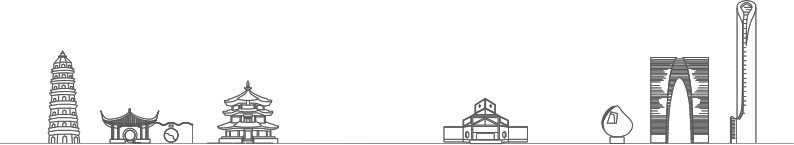
\includegraphics[width=\textwidth]{Cover_Suzhou.png}

    \vfill

    {\fontsize{12}{16}\selectfont\color{darkgray} 量子科技长三角产业创新中心\\编制：战略情报与成果专利室、产业发展部（理事会办公室）}
\end{center}
\end{titlepage}

% ==================== 目录 ====================
\pagenumbering{roman}
\newpage
\tableofcontents

\newpage

% ==================== 摘要 ====================
\pagenumbering{arabic}
\setcounter{page}{1}
\begin{center}
{\Large\bfseries\color{mainred} 摘\hspace{2em}要}
\end{center}
\addcontentsline{toc}{section}{摘要}


\textbf{ 宏观态势：}

全球量子科技正从研发布局转向规模化产业落地。法国追加10亿欧元、美国推出20亿美元激励计划，德国路线图强调产业化，凸显大国竞争加剧。量子安全成为紧迫议题，印度央行专设专家组评估加密转型，Synergy Quantum推出量子安全安卓系统，Bitcoin Cash完成抗量子升级。同时，量子计算基础设施加速部署，罗马尼亚、波兰引入本地量子计算机，欧洲推进全大陆QKD网络，反映出各国正从战略规划迈向实际建设与安全防御的双轨并进态势。


\textbf{ 科技前沿：}

量子计算硬件与材料研究取得多维突破。超导量子比特中观测到能量优势与混沌现象，金刚石超导机制新解有望催生多功能量子芯片。中性原子技术路径进展显著，实现原子与光子谐振器精准耦合，Pasqal验证逻辑量子比特在求解微分方程上优于物理比特。量子网络与通信方面，巴西启动永久性量子通信实验设施，散射介质被转化为安全传输新组件。此外，AI与量子深度融合，生成式AI用于量子线路合成，量子机器学习探索异常检测，开辟了算法与材料研究的新范式。


\textbf{ 产品动态：}

量子计算产品化与生态构建明显提速。中性原子领军企业Pasqal拟借壳上市，Quantum Machines实现跨平台全自动冷启动校准，甲骨文与Classiq合作推出AI驱动量子代码生成。在量子安全领域，后量子密码应用加速落地，Crypto4A发布密钥管理平台，GlobalPlatform推出开源芯片分发方案。同时，D-Wave升级超导量子比特材料制造，Rigetti采购先进蚀刻系统，Aegiq打造光子量子计算卓越中心，显示核心硬件制造能力正在向更高良率、更可集成化方向演进。


\textbf{ 企业资讯：}

本周企业动态虽少但指向关键资源整合。业界知名的量子计算先驱Seth Lloyd加入Planckian，专注于全局控制量子纠错策略，凸显顶尖人才向实用化纠错方案集中。PacketLight与Quantum XChange合作，将后量子密码与QKD融合强化光网络安全，表明网络设备商正主动整合多种量子安全技术。投资机构Ground State Ventures提升内部人才，反映量子基金对行业深度研判能力的重视，意在捕捉下一阶段增长机遇。三则动向共同指向技术深化与商用安全的融合趋势。


\textbf{ 资本运作：}

资本市场对量子计算的青睐持续升温。Quantinuum提交127亿美元估值IPO，Terra Quantum将以35亿美元估值通过SPAC上市，标志着量子独角兽进入公开市场。美国政府通过商务部渠道密集出手，拟向D-Wave、Rigetti、PsiQuantum等公司各提供高达1亿美元资助，并拨款3.75亿美元支持格芯建设量子技术解决方案部门。与此同时，Quanscient完成千万欧元A轮融资，SBQuantum获种子轮加速金刚石磁力计商业化，融资活动覆盖量子计算、传感与安全等细分赛道，显示资本正全方位注入量子产业链。






% ==================== 会议列表 ====================
{
    \newpage
    \section*{ 6月量子科技行业国内、国际会议}
    \addcontentsline{toc}{section}{ 6月量子科技行业国内、国际会议}
    \scriptsize
    \begin{longtable}{C{0.8cm}L{2.5cm}L{3cm}L{7cm}}
        \toprule[1.5pt]
        \textbf{序号} & \textbf{日期} & \textbf{地点} & \textbf{会议名称} \\
        \midrule
        \endfirsthead
        \toprule
        \textbf{序号} & \textbf{日期} & \textbf{地点} & \textbf{会议名称} \\
        \midrule
        \endhead
        \bottomrule
        \endfoot
        
        1 & 6月1日-3日 & 拉勒米, 美国 & 第四届怀俄明大学量子暑期学校 \\
        \midrule[0.05pt]
        
        2 & 6月1日-5日 & 罗利, 美国 & 2026量子机器学习暑期研讨会 \\
        \midrule[0.05pt]
        
        3 & 6月1日-5日 & 普罗维登斯, 美国 & 第57届APS原子、分子与光物理年会 \\
        \midrule[0.05pt]
        
        4 & 6月2日-4日 & 特隆赫姆, 挪威 & 量子自旋电子学 \\
        \midrule[0.05pt]
        
        5 & 6月3日-4日 & 罗切斯特, 美国 & 量子热力学与退相干 \\
        \midrule[0.05pt]
        
        6 & 6月4日-5日 & 东京, 日本 & Q2B：量子价值路线图 \\
        \midrule[0.05pt]
        
        7 & 6月5日 & 格拉斯哥, 英国 & 量子与社会研究研讨沙盒 \\
        \midrule[0.05pt]
        
        8 & 6月7日-12日 & 圣巴巴拉, 美国 & 第八届国际量子纠错会议 \\
        \midrule[0.05pt]
        
        9 & 6月7日-13日 & 克里特岛, 希腊 & 青年原子光学会议 \\
        \midrule[0.05pt]
        
        10 & 6月8日-11日 & 滑铁卢, 加拿大 & 量子光子学 \\
        \midrule[0.05pt]
        
        11 & 6月8日-20日 & 卡尔热斯, 法国 & 量子技术计算与通信暑期学校 \\
        \midrule[0.05pt]
        
        12 & 6月8日-8月14日 & 洛斯阿拉莫斯, 美国 & 2026洛斯阿拉莫斯量子计算暑期学校 \\
        \midrule[0.05pt]
        
        13 & 6月9日 & 巴黎, 法国 & Q-Day量子风险峰会：后量子密码学与量子密钥分发 \\
        \midrule[0.05pt]
        
        14 & 6月10日-12日 & 华沙, 波兰 & Perspektywy科技女性峰会 \\
        \midrule[0.05pt]
        
        15 & 6月10日-12日 & 多恩比恩, 奥地利 & 第四届砷化镓量子点国际研讨会 \\
        \midrule[0.05pt]
        
        16 & 6月10日-12日 & 埃朗根, 德国 & 神经形态计算前沿 \\
        \midrule[0.05pt]
        
        17 & 6月11日 & 杰克逊维尔, 美国 & 量子当下，医疗未来 \\
        \midrule[0.05pt]
        
        18 & 6月15日-17日 & 苏黎世, 瑞士 & 欧洲集成光学会议（ECIO） \\
        \midrule[0.05pt]
        
        19 & 6月15日-18日 & 格拉斯哥, 英国 & Optica Quantum 2.0会议 \\
        \midrule[0.05pt]
        
        20 & 6月15日-18日 & 赫尔辛基, 芬兰 & 仲夏开放量子系统、退相干及量子-经典交叉会议 \\
        \midrule[0.05pt]
        
        21 & 6月15日-18日 & 洛杉矶, 美国 & 量子器件设计研讨会 \\
        \midrule[0.05pt]
        
        22 & 6月16日 & 巴黎, 法国 & 第5届France Quantum \\
        \midrule[0.05pt]
        
        23 & 6月16日-17日 & 伦敦, 英国 & 第5届年度量子商业化全球大会2026 \\
        \midrule[0.05pt]
        
        24 & 6月16日-17日 & 格拉斯哥, 英国 & Optica 2026量子产业峰会——第5届 \\
        \midrule[0.05pt]
        
        25 & 6月21日-25日 & 塞费尔德, 奥地利 & 第57届欧洲原子系统组年度会议（EGAS 57） \\
        \midrule[0.05pt]
        
        26 & 6月21日-26日 & 塞费尔德, 奥地利 & 第7届塞费尔德量子信息研讨会 \\
        \midrule[0.05pt]
        
        27 & 6月21日-7月4日 & 贝纳斯克, 西班牙 & 量子科学：实现 \\
        \midrule[0.05pt]
        
        28 & 6月22日-24日 & 奥斯陆, 挪威 & IQT北欧：变化世界中的量子技术 \\
        \midrule[0.05pt]
        
        29 & 6月26日 & 汉堡, 德国 & 第7届ISC HPC国际研讨会——监控、可观测性与运营数据分析 \\
        \midrule[0.05pt]
        
        30 & 6月26日 & 汉堡, 德国 & 第2届统一计算中心量子资源研讨会（QRUCH） \\
        \midrule[0.05pt]
        
        31 & 6月26日 & 汉堡, 德国 & 第5届量子及混合量子/经典计算方法研讨会 \\
        \midrule[0.05pt]
        
        32 & 6月26日 & 汉堡, 德国 & 科学与工业数字孪生研讨会——从数据科学家到数据中心 \\
        \midrule[0.05pt]
        
        33 & 6月22日-7月3日 & 雷苏什, 法国 & 2026光子与原子暑期学校：量子气体、光-物质相互作用、量子技术 \\
        \midrule[0.05pt]
        
        34 & 6月23日-24日 & 罗马(纽约州), 美国 & 量子国际年度研讨会（Q4I） \\
        \midrule[0.05pt]
        
        35 & 6月23日-26日 & 阿尔加维, 葡萄牙 & 第3届量子安全网络与系统研讨会（QSNS 2026） \\
        \midrule[0.05pt]
        
        36 & 6月25日-26日 & 波士顿, 美国 & Quantum.Tech World \\
        \midrule[0.05pt]
        
        37 & 6月29日-7月1日 & 汉堡, 德国 & 国际计算科学大会量子计算专题 \\
        \midrule[0.05pt]
        
        38 & 6月29日-7月3日 & 贝桑松, 法国 & 第14届欧洲频率与时间研讨会（EFTS） \\
        \midrule[0.05pt]
        
        39 & 6月29日-7月10日 & 阿斯巴雷拉斯, 西班牙 & La Ricotta暑期学校：干草堆中的量子 \\
        \midrule[0.05pt]
        
        40 & 6月30日-7月1日 & 柏林, 德国 & GITEX欧洲 \\
        \midrule[0.05pt]
        
    \end{longtable}
}




% ==================== 宏观态势 ====================
\newpage
\section{宏观态势}
\vspace{-0.5em}
\noindent\rule{\linewidth}{1.5pt}

\subsection{ 揭示超导猫量子比特量子计算中的能量优势 }

2026年05月29日消息，超导量子比特量子计算机的能量效率研究取得进展。研究团队在猫量子比特平台上分析半经典量子傅里叶变换能量消耗，纳入纠错机制影响。结果显示，能量随量子比特数增加，通过优化参数可在保持保真度情况下最小化能耗。与经典计算机对比，假设卡诺效率，超26量子比特系统出现量子能量优势，考虑实际低温系统后依然成立。

\noindent\textbf{报道链接：}\url{https://arxiv.org/abs/2605.19854}

\subsection{ 构建欧洲量子盾牌：全大陆量子密钥分配（QKD）基础设施的战略视角 }

2026年05月29日消息，参考来源
➔
PDF下载
➔
量子计算的快速发展既能带来令人惊叹的科学突破，也可能被用于破解当今的安全系统，给现有数字体系带来新的风险。面对这一挑战，欧盟部署的欧洲通信基础设施（EuroQCI）至关重要。SEEWQCI项目融合了光纤电缆、卫星通信和增强型安全规则，构建起一道强大的数字屏障。其重点在于保护电网、医院等关键服务，保障欧洲民众的数据安全。

\noindent\textbf{报道链接：}\url{https://arxiv.org/abs/2605.22332}

\subsection{ 面向公用事业规模的多输出时间序列预测的混合量子-经典机器学习算法 }

2026年05月29日消息，IBM超导量子处理器上的多输出时间序列预测研究取得成果。第一种混合模型KQRC-RM使用114量子比特在MPS模拟器上MAE达0.0811，提升36.92\%；硬件上MAE为0.1524。第二种模型QGP用100量子比特，49\%输出高精度预测，低误差组平均MAE 0.082。相比经典GP基线，模拟器上平均MAE降低62.01\%，硬件降低40.37\%，证明100+量子比特NISQ设备可行性。

\noindent\textbf{报道链接：}\url{https://arxiv.org/abs/2605.24252}

\subsection{ 耗散猫量子比特中的比特翻转、饱和与量子混沌 }

2026年05月29日消息，玻色子猫量子比特研究揭示比特翻转饱和现象根源。通过量子轨迹模拟等分析，发现比特翻转是涉及存储器和缓冲器的动力学过程，锁相反射对称性破坏导致饱和。当绝热近似失效且存在交叉克尔相互作用等参数时，出现非规则动力学和混沌爆发，与实验数据吻合，揭示了耗散混沌对玻色子纠错的危害。

\noindent\textbf{报道链接：}\url{https://arxiv.org/abs/2605.24100}

\subsection{ 日本滨松光子学公司将在新加坡设立子公司以加强东南亚市场布局 }

2026年05月29日消息，日本滨松光子学公司近日宣布，它将在新加坡设立一家子公司以加强其在东南亚市场的业务基础。该子公司计划于2026年10月开始运营。未来，该公司将以这家新子公司为起点，致力于优化整个东南亚地区的供应链和服务结构，并计划随着区域市场的增长扩大其职能，以进一步强化其全球竞争力。

\noindent\textbf{报道链接：}\url{https://www.hamamatsu.com/us/en/news/announcements/2026/20260526000000.html}

\subsection{ Bitcoin Cash社区激活Layla升级 已加入后量子安全支持 }

2026年05月29日消息，Bitcoin Cash社区近日激活了Layla升级，引入了图灵完备的CashVM脚本语言，通过支持有限循环、函数、位运算及支付到脚本功能，拓展了Layer 1去中心化金融能力。此次升级还通过Quantumroot技术添加了后量子安全支持，OPTN Labs和Paytaca等钱包已在Android和iOS设备上为BCH、CashTokens及DeFi资产提供抗量子存储支持。该升级将推动新链上应用落地，包括去中心化交易所、永续合约交易、预测市场，以及基于x402支付协议的AI代理微支付等场景。

\noindent\textbf{报道链接：}\url{http://www.qtc.com.cn/flash/178001466033327.html}

\subsection{ 德国政府发布新版量子路线图：从研发转向产业规模化 }

2026年05月29日消息，德国联邦教育与研究部（BMFTR）近日正式发布了新版《量子技术路线图》，标志着德国量子政策正从研发向产业规模化发展向的关键转变。该国家量子路线图的核心支柱包括：在工业用例中实现可验证的量子优势以推动商业应用，构建关键子组件的弹性欧洲供应链确保可完全自主，培养具备市场技能的工程师队伍，以及利用“高科技空间”消除生态系统碎片化实现敏捷执行。这一框架将为德国量子技术的产业化落地提供系统性指导。

\noindent\textbf{报道链接：}\url{https://qbn.world/german-government-unveils-quantum-technologies-roadmap-for-its-hightech-agenda/}

\subsection{ Synergy Quantum宣布推出面向移动通信的量子安全安卓操作系统 }

2026年05月28日消息，Synergy Quantum近日宣布推出SynQ MobileOS Guard，这是一款面向移动通信场景的量子安全Android操作系统。该平台采用了经典密码学与后量子密码学的混合方案，以对设备端的语音、消息、信令及数据进行保护，并覆盖设备与所连接网络之间的通信链路。该混合加密架构将经典与后量子密码学相结合，使平台在应对当前安全威胁的同时，也具备抵御未来量子计算攻击的能力。其体系结构符合新兴国际后量子密码学标准方向，并与全球监管机构在移动通信量子安全准备方面的发展趋势保持一致。

\noindent\textbf{报道链接：}\url{http://quantumwire.com/article/17798438196494.html}

\subsection{ 波兰波兹南理工大学部署首台本地型量子计算机，欲推动量子教学与科研发展 }

2026年05月28日消息，波兰波兹南理工大学近日部署了由IQM量子计算公司提供的首台本地型量子计算机系统，以用于支持量子技术领域的教学与科学研究。据了解，该校部署的IQM Radiance R1系统与波兰量子技术发展路线图所设定的战略目标一致，同时也符合更广泛的欧洲相关倡议。校方表示，选择IQM方案的重要原因之一在于其可部署的本地化量子计算系统架构，使研究人员、学生与工程师能够在校园内直接访问真实的量子计算机。

\noindent\textbf{报道链接：}\url{http://quantumwire.com/article/17798424146491.html}

\subsection{ 罗马尼亚将投资超1亿欧元部署该国首台量子计算机 }

2026年05月27日消息，罗马尼亚计划于今年秋季在雅西部署该国首台量子计算机，总投资超过1亿欧元，并将向高校、研究机构及企业开放接入量子计算基础设施的能力。据悉，该项目旨在强化罗马尼亚的量子研究生态，其中罗马尼亚的亚历山德鲁·伊万·库扎大学将在量子技术相关的培训与研究项目中承担核心作用。研究人员表示，该量子计算系统可在网络安全、人工智能、物流、制药及先进材料等领域提供支持，通过执行复杂计算，解决传统计算机难以处理的问题。

\noindent\textbf{报道链接：}\url{https://thequantuminsider.com/2026/05/26/romania-plans-e100-million-quantum-computer-project-in-iasi/}

\subsection{ BitGo将与Silence Laboratories共同开发量子安全的MPC钱包基础设施 }

2026年05月27日消息，数字资产基础设施公司BitGo日前宣布达成一项战略合作，该公司将与Silence Laboratories共同开发面向机构数字资产托管与交易签名的量子安全多方计算（MPC）钱包基础设施。作为合作的一部分，双方已完成了首个由受监管托管机构基于MPC钱包基础设施进行的首次后量子交易模拟。该演示展示了一种全新的量子安全钱包架构，旨在帮助银行、托管机构、交易所及其他机构级数字资产平台，为后量子安全转型提供支持。

\noindent\textbf{报道链接：}\url{https://www.businesswire.com/news/home/20260526229210/en/BitGo-and-Silence-Laboratories-Complete-First-Post-Quantum-MPC-Transaction-Simulation-by-a-Regulated-Custodian}

\subsection{ 网络安全公司Genience宣布进军量子安全市场 }

2026年05月27日消息，网络安全公司Genience日前宣布进军量子安全市场，该公司计划为量子计算时代开发量子安全技术，并在后量子安全市场中确立自身定位。据相关人士透露，该公司“量子安全网关”技术已进入最终验证阶段，该技术属于其ZeroTrust 3.0战略的一部分。该技术旨在应对量子计算时代的黑客攻击威胁，并致力于构建自主知识产权、可与全球企业竞争的量子安全技术能力。

\noindent\textbf{报道链接：}\url{https://thequantuminsider.com/2026/05/26/genience-enters-4-7-trillion-won-quantum-security-market/}

\subsection{ ESL Shipping与QMill将合作探索量子计算在复杂航运决策领域的应用潜力 }

2026年05月27日消息，ESL Shipping近日启动了一项为期多年的研发项目“智能船队优化”，旨在探索量子计算在复杂航运运营中的应用，并通过先进优化方法提升船队层面的规划与决策能力。该项目得到芬兰国家商务促进局部分资助，将重点解决应对货物流动、运力约束、排放以及商业优先级同时管理所带来的挑战。在该项目中，ESL Shipping将与QMill合作，基于真实运营数据评估量子计算在优化问题中的适用性。

\noindent\textbf{报道链接：}\url{https://qmill.com/en/press-release-esl-shipping-and-qmill-explore-quantum-computing}

\subsection{ 印度储备银行新设Q-SAFE八人专家组，以全面评估量子威胁与加密转型 }

2026年05月26日消息，印度储备银行（RBI）日前宣布成立“量子安全与自适应金融生态系统专家委员会”（Q-SAFE），该委员会由八名成员组成，将负责评估量子技术在金融领域的潜在收益、风险与挑战。据悉，该委员会将通过加密材料清单（CBOM）评估金融行业的密码资产状况，分析加密敏捷性，并识别最易受到量子威胁影响的关键系统与流程。此外，该委员会还将评估行业对采用量子安全密码技术的准备程度，并为印度金融体系实现量子安全提出了路线图和框架建议。

\noindent\textbf{报道链接：}\url{https://www.thehindubusinessline.com/money-and-banking/rbi-launches-q-safe-panel-to-study-quantum-technology-in-banking/article71020966.ece}

\subsection{ 普林斯顿大学推出AI机器人实验室系统可实现石墨烯与量子材料自主制备 }

2026年05月26日消息，美国普林斯顿大学的研究人员开发出一款名为Qumus的AI驱动机器人实验室系统，可自主制备石墨烯，并制造包括石墨烯晶体管在内的原子级薄层量子材料器件。据介绍，该系统整合了大语言模型、机器人技术、计算机视觉与自动化实验设备，能够在无人干预条件下自主完成量子材料实验的规划、执行、分析与修正。他们的研究表明，此类自主实验系统有望加快量子材料、范德华结构及未来量子电子器件的发现与制造流程。

\noindent\textbf{报道链接：}\url{https://thequantuminsider.com/2026/05/25/ai-run-robot-lab-creates-graphene-and-builds-quantum-devices/}

\subsection{ 新加坡出台一系列新举措，助力企业应对AI革命与量子威胁双重挑战 }

2026年05月26日消息，新加坡近日宣布了多项新举措，旨在推动企业采用人工智能技术、提升网络韧性，并提前应对量子相关安全风险对电信基础设施带来的挑战。在ATxEnterprise 2026大会上，新加坡数字发展与信息部高级政务部长陈杰豪（音译）公布了“数字企业蓝图”下的新计划，该计划涉及与政府机构、科技公司及电信运营商的合作。这些措施旨在帮助新加坡企业借助AI提高竞争力，同时加强防御网络攻击的能力，并开始为后量子密码时代做准备，确保电信网络在量子计算威胁下仍能保存安全。

\noindent\textbf{报道链接：}\url{https://www.telecompaper.com/news/singapore-expands-quantum-safe-telecom-infrastructure-plans-enterprise-ai-initiatives--1571874}

\subsection{ 法国重金押注未来：马克龙宣布追加10亿欧元发展量子技术 }

2026年05月26日消息，法国总统马克龙于日前宣布，将追加15.5亿欧元（约17.9亿美元）投资量子计算与半导体领域，并指出欧洲各国应携手推进这两大关键战略技术，以在全球竞争中保持领先地位。在参观巴黎近郊的原子能暨替代能源委员会（CEA）超算中心时，马克龙透露，新资助方案将从“法国2030”计划中拨出10亿欧元用于量子技术，另增加5.5亿欧元支持半导体领域。这笔资金将助力量子计算领域的发展，并补充了法国于2021年投入18亿欧元以加强国家量子战略的承诺。

\noindent\textbf{报道链接：}\url{https://www.france24.com/en/live-news/20260522-france-announces-billion-euro-boost-for-quantum-computing}

\subsection{ 南卡罗来纳大学力邀前NASA及国土安全部专家，以加速量子信息技术布局 }

2026年05月25日消息，美国南卡罗来纳大学近日任命前NASA首席科学家Nasser Barghouty博士及前美国国土安全部新兴技术顾问Jalal Mapar担任高级外部顾问，任期数年，以拓展该校的量子信息科学与技术项目。未来两年内，两位顾问将支持应用量子研究、促进师生合作，并围绕南卡罗来纳州的量子生态与劳动力目标推进战略项目开发。此次任命基于该州2023年承诺的1500万美元量子准备资金，旨在将大学主导的研究与国家安全、基础设施及经济优先事项连接起来。

\noindent\textbf{报道链接：}\url{https://thequantuminsider.com/2026/05/21/university-of-south-carolina-establishes-national-level-quantum-senior-external-advisors-to-strengthen-research-and-education/}

\subsection{ 华东师大团队《自然》发文：量子增强电子隧穿 }

2026年05月25日消息，华东师范大学在《自然》发表研究，利用超快明亮压缩真空态驱动原子电子隧穿效应。实现超过20倍等效强度增强，即300纳焦脉冲能量相当于7.1微焦传统光。建立基于g(2)(0)的量子调控方法，并发展包含光电子纠缠的量子ADK理论。《自然》配发评论指出该工作提供明确量子优势。通讯作者吴健教授，倪宏程、蒋士成为共同通讯作者。

\noindent\textbf{报道链接：}\url{https://www.nature.com/articles/s41586-026-10485-9}

\subsection{ 美国伊利诺伊州发布该州首份量子教育全景报告 }

2026年05月25日消息，近日，美国伊利诺伊科技联盟、伊利诺伊经济发展公司、伊利诺伊量子与微电子园区以及芝加哥量子交易所发布了首份联合报告，系统追踪了伊利诺伊州量子人才培养体系的发展情况，进一步体现了该州在全美量子人才发展领域的领先地位。这份名为《伊利诺伊量子人才培养路径图谱：定义量子相关学位与证书的框架》的报告显示，2024年该州共颁发了超过33000个量子相关的学位与证书，较2018年《国家量子倡议法案》通过以来增长33\%，较过去十年累计增长60\%。该报告还指出，伊利诺伊州约占全美量子相关课程完成总量的近5\%。

\noindent\textbf{报道链接：}\url{https://iqmp.org/news/first-of-its-kind-report-positions-illinois-as-national-leader-in-quantum-workforce-development/}

\subsection{ 超导量子整机研发企业上海矩量光启获2亿元天使轮融资 }

2026年05月25日消息，最近，国内首家专注硅基衬底超导量子整机的企业上海矩量光启计算技术有限公司宣布完成2亿元天使轮融资，创下超导量子计算领域早期融资纪录。据悉，本轮融资由和利资本、钧山资本联合领投，中芯聚源（中芯国际旗下）、翌昕资本（长鑫存储关联方）等产业资本跟投，翊荣资本跟投并继续担任首席财务顾问，老股东千乘资本、德同资本及知名半导体设备方亦超额追加。

\noindent\textbf{报道链接：}\url{https://finance.sina.cn/tech/2026-05-18/detail-inhyhpys0834120.d.html}

\subsection{ 英国创新署量子PNT项目第一阶段结束，Xairos助力构建非GNSS授时体系 }

2026年05月24日消息，英国量子时间传递技术企业Xairos近日宣布，其参与的英国创新署“量子传感器与PNT任务先导”合同创新项目第一阶段已成功完成。在价值140万英镑的TimeLink计划支持下，Xairos主导完成了英国创新署量子PNT任务的第一阶段工作，降低了该公司专利量子协议的技术风险，并为英国建立了一套不依赖全球导航卫星系统（GNSS）的弹性授时硬件与软件基础。TimeLink第一阶段的成功收官，标志着英国在接受新一代授时技术方面迈出关键一步。

\noindent\textbf{报道链接：}\url{https://www.businesswire.com/news/home/20260521620579/en/Xairos-Closes-Out-Phase-1-of-the-Innovate-UK-Contracts-for-Innovation-Quantum-Sensors-and-PNT-Missions-Primer}

\subsection{ 美国政府宣布20亿美元量子计算激励计划，以强化在该领域的领导地位 }

2026年05月23日消息，美国商务部签署9份意向书，提供20.13亿美元联邦资金支持量子计算。代工厂格罗方德获3.75亿美元建立量子代工厂，IBM获10亿美元建立超导量子晶圆代工子公司。7家公司各获数千万至1亿美元，包括Atom Computing、Diraq、D-Wave、Infleqtion、PsiQuantum、Quantinuum及Rigetti，解决不同量子模式关键技术挑战。商务部将持少数股权。

\noindent\textbf{报道链接：}\url{https://www.nist.gov/news-events/news/2026/05/department-commerce-announces-letters-intent-9-companies-2-billion}


% ==================== 科技前沿 ====================
\newpage
\section{科技前沿}
\vspace{-0.5em}
\noindent\rule{\linewidth}{1.5pt}

\subsection{ 霍尼韦尔向英国最大室内光学设施交付一台可移动式地面光学站 }

2026年05月29日消息，霍尼韦尔交付可移动式地面光学站TOGS，支持英国萨福克学院量子光学发现实验室。该实验室是英国最大室内光学研究设施，可模拟大气条件测试激光通信。系统将与QEYSSat和霍尼韦尔QKDSat卫星测试，霍尼韦尔贡献约200万英镑投资。

\noindent\textbf{报道链接：}\url{https://www.satelliteevolution.com/post/honeywell-ground-optical-station-to-support-research-at-new-uk-quantum-space-optics-lab}

\subsection{ IBM 2026年Qiskit全球暑期学校现已开放注册 }

2026年05月29日消息，IBM日前表示，“2026年Qiskit全球暑期学校：云端十年”活动现已开放注册。该年度全球性项目旨在帮助学生、研究人员和开发者构建量子计算实用技能。为期两周的活动将于2026年7月13日至24日举行。这一免费在线课程将通过讲座、实验、IBM量子专家现场问答等环节，帮助学员使用Qiskit并掌握实用量子技能。要获得参与证书或徽章，学员需观看所有IBM量子核心讲座80\%的内容，高级赛道学员还需完成实验作业。

\noindent\textbf{报道链接：}\url{https://www.ibm.com/quantum/blog/qiskit-summer-school-2026}

\subsection{ 科学家在优化超导材料方面取得进展，新型缺陷识别将助力开发更低噪声量子器件 }

2026年05月29日消息，美国能源部的研究人员通过结合原子力显微镜、X射线和光谱分析等多种实验技术，深入探究了超导铌材料中缺陷的形成机制，并成功识别出一种名为“铌氢化物”的缺陷类型。这一发现意味着科学家现在可以有针对性地采取预防措施，例如通过优化材料和器件的工程化工艺，或在制造过程中更精准地控制器件所接触的气体，来抑制铌氢化物的生成。他们的研究结果表明，铌氢化物在铌薄膜中普遍存在，这为超导量子比特及其他谐振器中的退相干效应引入了一个此前未被考虑的因素。由于铌氢化物的尺寸、位置和密度会随器件从室温冷却的过程而变化，减少此类缺陷有助于降低量子计算机的噪声水平，从而使其在运行中减少错误。

\noindent\textbf{报道链接：}\url{https://www.energy.gov/science/hep/articles/spotting-new-culprit-hunt-quantum-noise}

\subsection{ 科学家将单个原子“钉”在光子谐振器旁，成功解决中性原子与集成光子学相结合难题 }

2026年05月29日消息，Quantum Source与魏茨曼科学研究所的研究人员近日成功将单个铷原子捕获在距离氮化硅光子谐振器表面仅150至200纳米的范围内，实现了原子与芯片上光场的强耦合。该实验解决了中性原子与集成光子学结合的关键难题：在平面芯片谐振器表面稳定捕获原子，同时避免其被表面吸附。该团队采用“单次加载”方法，通过光场减速接近的原子，并在一次散射事件后完成捕获，在最优条件下加载脉冲的捕获概率可达约30\%。捕获的原子会向谐振器发射光子，并表现出可测量的原子-光子耦合。这一成果为未来芯片集成量子光子系统提供了潜在的基础构建模块。

\noindent\textbf{报道链接：}\url{https://thequantuminsider.com/2026/05/27/researchers-trap-a-single-atom-on-a-photonic-chip-opening-a-route-to-integrated-quantum-optics/}

\subsection{ 巴西推进Quandanga量子通信网络项目，将建首个永久性实验基础设施 }

2026年05月29日消息，巴西国家电信局（Anatel）与军事工程学院（IME）近日举行了一次会晤，以讨论推进Quandanga量子通信网络项目的开发。该项目旨在打造巴西首个永久性实验基础设施，用于研究、测试和演示基于量子及后量子密码技术的安全通信方案。这一合作标志着巴西在量子通信领域迈出关键一步，未来将为该国在量子安全通信的技术验证与标准化方面提供长期实验平台。

\noindent\textbf{报道链接：}\url{https://www.telecompaper.com/news/brazil-plans-development-of-quantum-communication-network--1572267}

\subsection{ QuantumCT联合康涅狄格大学与耶鲁大学启动新一阶段试点项目以推动量子创新 }

2026年05月28日消息，康涅狄格量子技术计划（QuantumCT）日前宣布，它与美国康涅狄格大学及耶鲁大学合作推进的四项第二阶段试点项目已正式启动。这些项目由康涅狄格大学、耶鲁大学及产业合作伙伴共同资助，将依据其在应用量子研究方面的推进能力进行遴选，重点面向康涅狄格州具有战略意义的产业领域，包括航空航天与国防、高端制造、金融服务、保险及生命科学。该批项目是在第一阶段试点计划成功基础上的延续。第一阶段主要支持量子算法、硬件集成、量子传感及应用计算等方向的早期概念验证研究。

\noindent\textbf{报道链接：}\url{http://quantumwire.com/article/17798495246501.html}

\subsection{ 莫纳什大学开发的纳米电路可在单一芯片上实现光信息生成、引导与读取 }

2026年05月28日消息，澳大利亚莫纳什大学的研究人员开发出一种纳米尺度电路技术，可在单一芯片上实现光信息的生成、引导与读取。通过结合先进材料与纳米技术，这种方法解决了“谷电子学”领域的一项长期挑战。该领域被认为有望用于更高速、更高能效的计算及量子技术发展。据介绍，研究人员首次展示了一个完全集的成系统，可在紧凑芯片器件中生成特定光信号、实现精确引导，并将其转换为电信号。相关研究成果已于日前发表在《自然·光子学》期刊。

\noindent\textbf{报道链接：}\url{http://quantumwire.com/article/17798458856498.html}

\subsection{ 美国科学家开发的新型声学器件可简化量子传感器设计 }

2026年05月27日消息，美国加州理工学院与斯坦福大学的研究人员开发出一种名为“纳米机电系统”（NEMS）的器件，可使声子仅依靠器件材料自身的内在特性展现量子行为。此前，这类量子行为通常需要借助超导量子比特等外部量子器件才能实现观测。该研究表明，基于这一新机制，单个NEMS器件即可作为结构更简化、更紧凑的量子传感器或量子比特使用。据研究人员称，该成果是量子声学领域的最新进展，推动了基于单个声子的量子传感技术发展，为高精度探测材料中的极微小变化提供了新的技术路径。相关研究成果已于日前发表在《自然·物理》期刊。

\noindent\textbf{报道链接：}\url{https://www.caltech.edu/about/news/tuning-into-quantum-sounds}

\subsection{ 日本科学家发现将分子与量子点组合可显著提升太阳能电池效率 }

2026年05月27日消息，日本大阪大学及其合作机构的研究人员揭示了一种新的机制，通过将特定设计的分子与量子点进行组合，可以显著提升太阳能电池的效率，并有望突破当前太阳能电池的效率上限。这一成果被认为为提升太阳能技术对光能的利用效率提供了新的路径。相关研究成果已于日前发表在《自然·光子学》期刊。

\noindent\textbf{报道链接：}\url{https://phys.org/news/2026-05-supercharging-solar-cells-quantum-dot.html}

\subsection{ 北京量子院研究团队利用生成式AI实现连续原生门量子线路的混合扩散-优化合成 }

2026年05月26日消息，北京量子信息科学研究院利用生成式AI实现连续原生门量子线路优化合成。开发混合扩散优化框架，将去噪扩散模型与梯度优化结合。对10000个随机三比特幺正矩阵测试，能生成良好近似线路。模型可学习连续参数分布，适应不同硬件原生门集，论文发表于Physica Scripta，第一作者郭大钧，通讯作者苏晓禄。

\noindent\textbf{报道链接：}\url{https://iopscience.iop.org/article/10.1088/1402-4896/ae6a4a}

\subsection{ 浙江大学量子物态与器件研究中心：耗散塑造响应 }

2026年05月26日消息，浙江大学施李坤、常凯团队在非线性量子输运理论获进展。论文发表于Physical Review Letters并被选为封面。研究揭示非线性响应中耗散机制参与塑造量子几何，通常的内禀响应包含两部分，除量子几何外还有纯动力学贡献。不存在与环境无关的普适内禀公式，解释不同实验差异。第一作者郭智超。

\noindent\textbf{报道链接：}\url{https://journals.aps.org/prl/abstract/10.1103/rbck-mt1k}

\subsection{ 南京大学邹欣晔和程建春课题组实现轨道诱导的三维ℤ分类高阶拓扑绝缘体 }

2026年05月26日消息，南京大学邹欣晔、程建春课题组在高阶拓扑声学取得进展，发表于Physical Review Letters。首次在三维声学晶体中实验实现ℤ分类高阶拓扑绝缘体，利用简并p轨道构建三维SSH模型。观测到24个带隙内拓扑角态，对应8个角点各3个态，实现轨道选择性调控的拓扑相变。

\noindent\textbf{报道链接：}\url{https://journals.aps.org/prl/abstract/10.1103/74kx-xg78}

\subsection{ Quantum Midi Posse在IBM硬件上完成一项基准测试，成功验证其QSCE框架 }

2026年05月26日消息，Quantum Midi Posse日前公布了一项在IBM Marrakesh超导量子系统上完成的基于96个活跃量子比特的基准测试。此次测试在未采用量子纠错或后选择机制的条件下进行，该公司表示，其结构化输出模式在原生桥接NISQ执行过程中仍得以保留。测试重点验证了其专有的量子态指令编码（QSCE）框架。实验基于六个同时运行的16量子比特区域展开，并通过原生跨区域桥接操作实现互联。结果显示，结构化量子输出在多种控制配置下仍具有可区分性。

\noindent\textbf{报道链接：}\url{https://thequantuminsider.com/2026/05/24/quantum-midi-posse-reports-96-qubit-structured-output-benchmark-on-ibm-hardware/}

\subsection{ 从障碍到资源：卡尔斯鲁厄理工学院首次实现对超导体磁涡旋进行量子控制 }

2026年05月26日消息，德国卡尔斯鲁厄理工学院（KIT）的一个研究团队最近通过实验证明，超导体中此前被视为干扰因素的磁涡旋，可在特定材料中被用来作为可控量子系统。他们的这一发现将原本不受欢迎的物理现象转化为了量子技术中的一种潜在资源，为量子计算机、高灵敏度传感器系统及材料科学创新方法的发展开辟了新路径。相关研究成果已于近日已发表在《自然》杂志上。

\noindent\textbf{报道链接：}\url{https://www.kit.edu/kit/english/pi\_2026\_046\_once-a-disruption-now-a-resource-superconducting-vortices-used-as-qubits.php}

\subsection{ 研究人员利用经典计算机成功求解被认为不可能完成的复杂量子物理问题 }

2026年05月26日消息，来自西蒙斯基金会熨斗研究所计算量子物理中心（CCQ）以及美国波士顿大学的物理学家，利用传统计算机结合先进数学工具与程序代码，成功求解了一个此前被认为只能由量子计算机才能解决的复杂量子物理问题。该方法在计算效率上实现突破，使研究人员甚至能够在个人笔记本电脑上完成求解。这一方法提升了经典计算机在复杂问题求解方面的能力，为量子动力学研究开辟了新的方向，并可能为在大量可行解中寻找最优解的问题提供一种参考性求解范式。相关研究成果已于日前发表在《科学》期刊。

\noindent\textbf{报道链接：}\url{https://www.simonsfoundation.org/2026/05/21/quantum-dynamics-breakthrough-overturns-claim-of-quantum-supremacy-opens-new-research-directions/}

\subsection{ OIST新研究重新定义自旋玻璃，为量子自旋液体提供了更稳健研究路径 }

2026年05月26日消息，近日，日本冲绳科学技术大学院大学（OIST）电子与量子磁学课题组的研究人员在实验中观测到，在逐步引入化学无序的过程中，高度有序的反铁磁晶体中自旋组织发生的演化行为。基于该结果，研究人员对“自旋玻璃”这一概念给出了实验验证定义，为其提供了更清晰的解释框架，并有助于更准确地解读相关实验研究结果。此前，自旋玻璃在理论物理与材料科学之间存在一定认知差异。这一重新定义也为研究量子自旋液体提供了一种更为稳健的研究路径。相关研究成果已于日前发表在《Matter》期刊。

\noindent\textbf{报道链接：}\url{https://www.oist.jp/news-center/news/2026/5/21/complete-evolution-spin-glass-order-chaos}

\subsection{ 德国科学家成功实现对有机分子进行单分子级的量子调控 }

2026年05月26日消息，来自NVision成像技术公司和德国乌尔姆大学等机构的科学家们报告称，单个有机分子在光作用下可实现量子信息的存储、操控与读取，并演示了对单个有机分子的相干量子控制与光学读出。该研究指出，这一结果提示了一种潜在的量子技术路径，可通过化学工程设计的分子体系构建量子器件，而非依赖传统半导体缺陷结构。此外，该研究还展示了一种单分子自旋-光子接口，在特殊设计的晶体中嵌入有机卡宾分子，这使分子量子系统从传统的多分子集合实验推进至单分子层级的控制。相关研究成果已于日前发表在预印本平台arXiv上。

\noindent\textbf{报道链接：}\url{https://thequantuminsider.com/2026/05/20/molecular-qubit-achieves-single-photon-quantum-control/}

\subsection{ WISER与弗劳恩霍夫的新联合研究探索了量子机器学习在异常检测中的应用 }

2026年05月25日消息，美国华盛顿WISER研究所与德国弗劳恩霍夫工业数学研究所（Fraunhofer ITWM）近日在WISER量子与人工智能计划下完成一项联合研究项目，推动了对量子机器学习在工业实际应用场景中的理解。该合作的核心是探索新兴量子计算方法如何支持制造业中的异常检测，这一任务对于识别复杂生产系统中的故障至关重要。通过分析工业设备中的传感器数据，这类方法旨在及早发现异常，从而减少停机时间、提升质量控制并提高整体效率。这项工作成功展示了量子机器学习如何在当下解决实际工业问题，同时揭示了随着量子硬件的不断发展，其有望提升复杂生产环境中决策支持质量的潜力。

\noindent\textbf{报道链接：}\url{https://www.itwm.fraunhofer.de/en/press-publications/press-releases/2026/2026\_05\_19\_WISER\_EN.html}

\subsection{ 科学家化障碍为利器：散射介质可变身为量子信息安全传输新组件 }

2026年05月25日消息，来自法国巴黎纳米科学研究所、法国卡斯特勒-布罗塞尔实验室以及英国格拉斯哥大学的研究人员联合开发出一种新方法，能使散射介质仅对纠缠光子对所携带的信息保持透明，而对经典光仍完全不透明。据团队介绍，他们通过将光学无序结构转化为可区分经典信息与量子信息的选择性滤波器，实现了一项重要概念突破——复杂介质不再只是量子信息传输中的干扰因素，而可作为具备主动调控能力的可编程功能组件。研究人员指出，这种基于物理机制的信息区分能力，在安全通信领域具有广阔应用前景。相关研究成果已于日前发表在《光学》和《自然·物理》期刊。

\noindent\textbf{报道链接：}\url{https://www.lkb.fr/en/the-quantum-key-to-seeing-through-chaos/}

\subsection{ 金刚石超导机制获新解：美研究人员为开发多功能量子芯片奠定了基础 }

2026年05月25日消息，近日，来自美国宾夕法尼亚州立大学、芝加哥大学普利兹克分子工程学院以及由美国阿贡国家实验室牵头的美国能源部国家量子信息科学研究中心Q-NEXT的研究人员，通过制备高质量金刚石，并从材料噪声中分离电子信号，揭示了金刚石中超导现象背后的物理机制新见解。这一发现为在同一量子芯片上实现多种功能提供了潜在路线图，该创新有望提升量子技术效率，并增强其与经典技术的集成能力。相关研究成果已于日前发表在《美国国家科学院院刊》上。

\noindent\textbf{报道链接：}\url{https://pme.uchicago.edu/news/designer-superconducting-diamond-researchers-uncover-path-multi-modality-quantum-chips}

\subsection{ 中国科大发现镍基高温超导机制的重要实验证据 }

2026年05月25日消息，中国科学技术大学何俊峰与南方科技大学薛其坤、陈卓昱合作在镍基高温超导获突破，成果发表于《科学》。在(La,Pr,Sm)3Ni2O7薄膜中直接观测到无节点超导能隙及\textasciitilde{}70 meV处能带扭折，揭示s波对称性及电子玻色子耦合。联合研发液氮超高真空低温淬火传输技术。共同第一作者沈建昌等，共同通讯何俊峰、薛其坤、陈卓昱。

\noindent\textbf{报道链接：}\url{https://www.nature.com/articles/s41586-025-08755-z}

\subsection{ 法国团队突破性研究：利用量子纠缠实现不透明介质透明化 }

2026年05月24日消息，法国团队包括CNRS科学家实现利用量子纠缠使不透明介质透明。纠缠光子穿越无序介质时保持相干性，图像信息可保存，经典光则会被破坏。发现发表于《自然·物理学》，为散射介质信息传输提供新思路，有望应用于安全通信和医学成像。

\noindent\textbf{报道链接：}\url{https://www.cnrs.fr/en/press/rendering-opacity-transparent-through-quantum-entanglement}

\subsection{ Pasqal首次在真实量子处理器上验证逻辑量子比特要显著优于传统方法 }

2026年05月24日消息，Pasqal近日宣布取得一项最新研究成果，展示了量子计算在解决实际问题上的显著进步。该公司首次在真实硬件上验证了“逻辑量子比特”在求解微分方程时优于标准量子计算技术。相关研究已发表于arXiv平台。Pasqal是使用其量子处理器求解微分方程，这类方程是能源系统、材料科学和金融建模等众多实际应用的核心基础。结果显示，逻辑量子比特方法相比传统方法平均性能提升超过50\%，在特定难题上性能提升高达十倍。值得注意的是，尽管逻辑量子比特方法更为复杂，但它仍能实现这一提升，凸显了其实际应用价值。

\noindent\textbf{报道链接：}\url{https://beian.miit.gov.cn}

\subsection{ Pasqal首次利用中性原子量子计算机演示逻辑比特在求解微分方程方面要强于物理比特 }

2026年05月23日消息，Pasqal宣布在中性原子处理器上证明逻辑量子比特方法优于标准方法，求解微分方程。平均性能提升超50\%，某些问题提升十倍。研究使用99.4\%门保真度硬件运行1000个方程比较。逻辑量子比特天然抵抗特定噪声，结果发表于arXiv。首席技术官Loïc Henriet称这是PROQCIMA计划直接产物。

\noindent\textbf{报道链接：}\url{https://www.pasqal.com/newsroom/pasqal-demonstrates-logical-qubits-outperform-physical-qubits-solving-differential-equations-an-industry-first-for-neutral-atom-quantum-computing/}


% ==================== 产品动态 ====================
\newpage
\section{产品动态}
\vspace{-0.5em}
\noindent\rule{\linewidth}{1.5pt}

\subsection{ 北京量子院团队提出ZAP方案，可破解中性原子量子芯片原子搬运与串扰控制等难题 }

2026年05月29日消息，北京量子信息科学研究院量子操作系统软件研发团队提出一种面向场可编程原子阵列的分区架构与高性能编译框架ZAP。该工作通过硬件架构与编译算法协同设计，解决了中性原子量子计算中逻辑线路映射、原子搬运、串扰控制与编译效率之间的关键矛盾。相关成果已于日前在线发表于《电气与电子工程师协会量子工程汇刊》。

\noindent\textbf{报道链接：}\url{https://www.baqis.ac.cn/news/detail/?cid=4688}

\subsection{ Quantum Machines实现7天冷启动Rigetti量子处理器，且性能达到官方调控水平 }

2026年05月29日消息，Quantum Machines使用OPX1000平台在7个工作日内将Rigetti Novera QPU从冷启动调至全面运行。在11对量子比特上实现双量子比特门中值保真度99.5\%，峰值99.86\%。单量子比特门中值保真度99.93\%，读取保真度95\%。代表外部编排平台实现最高Novera全系统性能。

\noindent\textbf{报道链接：}\url{https://www.quantum-machines.co/blog/rigetti-novera-99-5-fidelity-opx1000/}

\subsection{ 甲骨文与Classiq合作完成由AI驱动的量子代码生成与大规模仿真验证 }

2026年05月29日消息，甲骨文公司与量子软件工程平台开发商Classiq近日合作完成了一项高性能计算概念验证，成功将自然语言人工智能生成与大规模经典仿真集群相结合。该端到端软件工作流展示了AI代理如何根据抽象的用户提示，综合生成企业级量子代码，并自动编译成可执行电路。为验证程序的规模化运行能力，该团队将计算任务路由至甲骨文云基础设施上的NVIDIA DGX A100超级计算节点，成功执行了一项超出标准本地开发环境极限的36量子比特仿真任务。

\noindent\textbf{报道链接：}\url{https://quantumcomputingreport.com/oracle-and-classiq-integrate-quantum-ai-agents-with-oci-for-36-qubit-portfolio-optimization-hpc-simulation/}

\subsection{ 中性原子量子计算公司Pasqal拟借壳上市，已提交业务合并注册声明 }

2026年05月28日消息，Pasqal与Bleichroeder Acquisition Corp. II向SEC提交F-4联合注册声明，推进业务合并。Pasqal在中性原子量子计算领域拥有最多部署量，7台QPU交付，3台生产中。投前估值20亿美元，预计总收益5亿美元。路线图目标2029年底每QPU超10000物理量子比特和超200逻辑量子比特。创始人包括诺奖得主Alain Aspect。

\noindent\textbf{报道链接：}\url{https://www.globenewswire.com/news-release/2026/05/26/3301476/0/en/pasqal-and-bleichroeder-acquisition-corp-ii-announce-filing-of-registration-statement-on-form-f-4-in-connection-with-proposed-business-combination.html}

\subsection{ Pasqal已与特殊目的收购公司联合向美国证券交易委员会提交F-4表格注册声明 }

2026年05月28日消息，法国中性原子量子计算公司Pasqal已与美国特殊目的收购公司（SPAC）Bleichroeder Acquisition Corp. II联合向美国证券交易委员会提交了F-4表格注册声明，其中包括一份初步的代理声明/招股说明书。此举是双方于2026年3月4日宣布的拟议业务合并进程中的关键里程碑。Pasqal目前是全球纯量子计算企业中拥有最多高量子比特数量子计算机安装量的公司之一，此次合并将有助于加速其高性能硬件与云就绪软件解决方案的开发。

\noindent\textbf{报道链接：}\url{http://quantumwire.com/article/17798528886506.html}

\subsection{ Qubic与Quantum Machines签署合同，其低温放大器迎来首个客户 }

2026年05月28日消息，加拿大量子硬件开发商Qubic近日宣布，其已与量子计算混合控制系统开发商Quantum Machines签署一份合同，后者成为了其低噪声低温放大器产品的首个客户。根据协议，双方将合作探索把Qubic的低温放大器集成至量子计算技术栈中，以提升量子计算机性能。作为集成合作伙伴，Quantum Machines将率先获得该技术的早期访问权限，其内部团队也将对该放大器开展评估、基准测试，并与现有解决方案进行详细比较。

\noindent\textbf{报道链接：}\url{http://quantumwire.com/article/17798524656505.html}

\subsection{ GlobalPlatform推出集成了后量子密码技术的开源硅芯片分发方案 }

2026年05月28日消息，GlobalPlatform近日发布了开源硅芯片分发方案Pavona。据了解，该方案能提供生产级、可认证的IP组件与参考顶层设计，它包含首个公开可用的嵌入式芯片后量子密码（PQC）软件栈，并提供两项已完成流片的参考设计：包括独立芯片信任根以及面向小芯片架构的集成式信任根。这些设计均基于台积电3nm（N3）工艺制造。Pavona旨在提供可组合框架，用于构建默认安全的芯片设计体系，并对齐FIPS 140-3及通用标准认证要求。

\noindent\textbf{报道链接：}\url{http://quantumwire.com/article/17798511496503.html}

\subsection{ D-Wave获NORDTECH第二年项目资金支持，将推动超导量子比特材料制造升级 }

2026年05月28日消息，D-Wave日前宣布，它已获得美国东北区域国防技术中心（NORDTECH）资助的“利用可扩展制造工艺改进超导量子比特材料（SQFab）”项目的第二年资金支持。据悉，该项目属于四个相关项目之一。这四个项目在完成第一年关键指标并在量子计算关键组件的设计、制造与表征方面取得重要进展后，合计获得了超过2500万美元的第二年资金支持。D-Wave表示，其参与的SQFab项目旨在通过可扩展制造方法改进超导量子比特材料，以推动下一代微电子能力从科研阶段向制造阶段发展。

\noindent\textbf{报道链接：}\url{http://quantumwire.com/article/17798500716502.html}

\subsection{ ORCA Computing与Digital Realty合作，探索量子加速与AI基础设施融合 }

2026年05月28日消息，ORCA Computing近日宣布参与Digital Realty在伦敦新推出的DRIL创新实验室，该实验室由全球最大的云和运营商中立数据中心提供商Digital Realty打造，是一个面向下一代基础设施的测试环境。此次合作标志着ORCA在商业化进程中取得重要进展，随着企业越来越多地探索量子加速如何与AI及高性能计算基础设施融合，ORCA的PT系列光子量子系统将在实验室的实际环境中与领先的AI和基础设施技术协同运行，且无需专门冷却或特殊基础设施支持。

\noindent\textbf{报道链接：}\url{http://quantumwire.com/article/17798461726499.html}

\subsection{ Telia Finland与QMill联合开发面向移动网络的量子增强消息加密技术 }

2026年05月28日消息，Telia Finland与QMill最近联合开发了一种面向移动网络的量子增强消息加密技术。该加密方法由QMill提出，可通过本地或云端量子计算机实现，部署后旨在保护通信消息免受基于经典计算资源或量子计算资源的攻击。这一技术演示是对Telia既有成果的补充。此前，Telia已在其网络中成功测试量子密钥分发（QKD）技术，成为了芬兰首个完成此类测试的商业运营商，而该QKD测试属于芬兰国家量子安全网络项目NaQCI.fi的一部分。

\noindent\textbf{报道链接：}\url{http://quantumwire.com/article/17798452466496.html}

\subsection{ SeQure Quantum成功在智利部署一条量子安全通信链路 }

2026年05月27日消息，SeQure Quantum公司日前宣布，已在智利国家电力协调局与该国一家电力行业运营机构之间成功部署一条量子安全通信链路。该系统集成了量子随机数生成器（QRNG）、后量子密码学（PQC）以及高安全性网络加密设备等技术。据悉，此次部署在Thales集团的支持下完成了验证，并由Dreamlab Technologies进行独立评估，旨在展示智利在能源、电信、金融、水务和国防等关键领域构建与运行具有量子安全的网络安全系统的能力。

\noindent\textbf{报道链接：}\url{https://thequantuminsider.com/2026/05/25/sequre-quantum-the-first-quantum-safe-link-in-critical-electrical-infrastructure-in-chile/}

\subsection{ 拉西瑞亚大学与enQase正合作推进量子安全基础设施部署 }

2026年05月27日消息，美国拉西瑞亚大学与enQase正合作推进量子安全基础设施部署，以应对未来量子计算可能带来的安全威胁，从而保护大学系统与数据安全。双方的合作聚焦于关键网络连接与密码系统防护，采用后量子加密、量子密钥分发以及量子随机数生成等技术，并结合美国国家标准与技术研究院（NIST）的迁移时间表推进相关安全升级。enQase的首席执行官Rajesh Patil表示，该项目使拉西瑞亚大学成为了美国较早推进量子安全校园网络部署的高校之一。

\noindent\textbf{报道链接：}\url{https://lasierra.edu/article/la-sierra-university-launches-futuristic-quantum-secure-pilot-to-protect-data/}

\subsection{ 英国量子计算初创公司Universal Quantum受到多家SPAC公司关注 }

2026年05月27日消息，英国量子计算初创公司Universal Quantum最近受到多家美国投资机构提出的收购与上市意向，这正值英美两国在商用量子计算领域的竞争日趋激烈之际。据外媒报道，多家美国特殊目的收购公司（SPAC）已与这家位于布莱顿的初创企业接洽，讨论其在纽约证券交易所上市的可能性。与此同时，Universal Quantum正寻求最高达1亿美元融资，投资方包括硅谷风险投资机构。该资金将用于开发可连接多个量子芯片的系统，以推动构建更大规模、更高性能的量子计算机。

\noindent\textbf{报道链接：}\url{https://thequantuminsider.com/2026/05/26/uk-quantum-startup-draws-interest-from-u-s-spacs-the-telegraph-reports/}

\subsection{ Scaleway与QbitSoft联手推出欧洲首个云原生量子采用计划 }

2026年05月26日消息，欧洲公有云服务提供商Scaleway与法国量子应用深科技公司QbitSoft日前联合推出“量子采用计划”，旨在帮助企业识别、验证并扩展量子技术应用场景，同时降低量子技术使用门槛，无需企业具备相关前期专业经验。该计划整合了主权云平台、应用专业知识以及对多种量子技术的直接访问能力，提出了一种面向欧洲市场的量子技术应用模式，重点基于云原生架构，并聚焦实际业务应用与落地。

\noindent\textbf{报道链接：}\url{https://www.scaleway.com/en/news/scaleway-and-qbitsoft-launch-europes-first-cloud-native-quantum-adoption-program/}

\subsection{ Crypto4A正式发布量子安全密钥管理平台QxVault }

2026年05月26日消息，Crypto4A日前宣布其新一代密钥与敏感信息管理平台QxVault正式商用。该平台基于Crypto4A的量子安全架构，并以符合FIPS 140-3 Level 3i认证的加密模块为核心支撑，在提供企业级安全防护能力的同时降低了传统方案的运维负担。QxVault面向企业及政府机构，旨在以更简化的方式实现对敏感数据的安全保护，并提升可控性与面向未来的安全能力。随着组织逐步从分散的安全架构与复杂的传统工具体系转型，该平台提出了统一方法，通过量子安全平台简化密钥管理流程，并强化了数字信任基础。

\noindent\textbf{报道链接：}\url{https://www.prnewswire.com/news-releases/crypto4a-announces-general-availability-of-qxvault-a-quantum-safe-secrets-management-platform-built-for-simplicity-sovereignty-and-scale-302780466.html}

\subsection{ Rigetti采购牛津仪器的原子层蚀刻系统，以提升其量子晶圆厂制造能力 }

2026年05月25日消息，牛津仪器（Oxford Instruments）近日宣布，量子计算公司Rigetti Computing已购买其PlasmaPro 100 Cobra原子层刻蚀（ALE）系统，用于量子器件的专用制造，以进一步提升其近期扩建的量子代工厂。牛津仪器表示，该公司的ALE技术可为下一代量子器件提供平滑、低损伤的刻蚀工艺，使PlasmaPro 100 Cobra成为了Fab-1量子制造工厂的理想选择。Rigetti开创的量子代工模式还证明了在规模化提升质量和性能的过程中，投资内部量子比特制造能力的价值。

\noindent\textbf{报道链接：}\url{https://www.oxinst.com/news/oxford-instruments-to-supply-atomic-layer-etch-equipment-to-rigetti-computing-to-expand-advanced-quantum-fabrication-capabilities/}

\subsection{ Aegiq启用英国新总部，计划投数百万英镑打造光子量子计算卓越中心 }

2026年05月25日消息，英国量子技术公司Aegiq近日在谢菲尔德启用新总部，以建立专注于光子量子计算的卓越中心。该公司计划在未来五年投资数百万英镑，重点面向毕业生和早期职业人才创造高技能岗位。Aegiq将借助英国在光子学与半导体制造领域的优势，致力于开发可扩展的量子计算机，应用可覆盖航空航天、网络安全和医疗健康领域，此举旨在将英国南约克郡打造为这一新兴技术的核心枢纽。

\noindent\textbf{报道链接：}\url{https://quantumzeitgeist.com/aegiq-plans-multi-million-pound/}

\subsection{ QuiX发布光子组装控制单元 可降低光量子系统复杂度并提升集成与维护效率 }

2026年05月25日消息，QuiX Quantum近日推出新型光子组装控制单元（PACU），为其光量子系统及未来通用量子计算机构建了可扩展、标准化的控制层。据该公司称，PACU采用机架式架构，支持最多1000个低速和32个高速移相器，响应时间低于2毫秒，并集成以太网与USB连接、空气冷却、过热保护以及光子组件热插拔等功能。QuiX Quantum公司表示，随着光子量子系统逐步迈向更广泛的工业与商业应用，PACU有助于降低系统运行复杂度，并提升模块化能力、维护效率及数据中心集成水平。

\noindent\textbf{报道链接：}\url{https://www.quixquantum.com/news/quix-quantum-introduces-pacu-a-photonic-assembly-control-unit-for-scalable-quantum-systems}

\subsection{ SBQuantum获得加拿大国防部两份价值300万加元的量子磁力计合同 }

2026年05月25日消息，SBQuantum日前宣布获得两项总金额达300万加元的新合同。据了解，该公司为首家提供量子金刚石磁力计的企业，其技术可在公共安全、导航及国防等领域提供高精度实时数据支持。这两项合同获得了加拿大政府创新项目支持，并与加拿大国防部相关优先事项保持一致，将推动SBQuantum向国防相关环境交付其专有量子磁力计阵列，以用于测试与验证。在项目执行过程中，该公司将部署量子传感器阵列，并与其磁信息平台协同使用，后者集成了噪声消除算法与实时分类能力。这些技术将应用于磁导航、铁磁性金属物体探测以及隐蔽行动等多种场景。

\noindent\textbf{报道链接：}\url{https://www.einpresswire.com/article/913857794/sbquantum-announces-two-new-contracts-with-canada-s-department-of-national-defence-totaling-3-million?n=2}

\subsection{ Superpositions Studio推出面向企业的量子机器学习平台 }

2026年05月24日消息，Superpositions Studio云量子机器学习与优化平台近日宣布结束早期访问计划，正式推出通用版本。该平台通过提供无代码、AI辅助的界面，使企业能够在多个硬件提供商之间测试量子与混合工作流。Superpositions Studio支持量子与经典方法的基准对比，应用场景涵盖金融、能源、制造、物流与医疗等领域。

\noindent\textbf{报道链接：}\url{https://thequantuminsider.com/2026/05/20/superpositions-studio-general-availability-quantum-ml-platform/}

\subsection{ 后量子密码学护航AI机器人：WISeKey推出WISeRobot.ch平台应对量子威胁 }

2026年05月24日消息，WISeKey与SEALSQ近日联合推出WISeRobot.ch平台，该平台专注于以人为中心的机器人技术，并采用后量子密码学进行安全防护。两家公司正将后量子半导体、公钥基础设施（PKI）及数字身份系统集成至AI驱动的机器人平台中。此次发布是WISeKey战略的关键一步，旨在将抗量子安全能力直接嵌入下一代机器人系统，以应对量子计算发展带来的新兴安全风险。

\noindent\textbf{报道链接：}\url{https://www.sealsq.com/investors/news-releases/sealsq-and-wisekey-announce-roadmap-and-launch-of-official-website-for-wiserobot.ch-integrating-human-centric-ai-with-post-quantum-securi-1779260403116}




% ==================== 企业资讯 ====================
\newpage
\section{企业资讯}
\vspace{-0.5em}
\noindent\rule{\linewidth}{1.5pt}

\subsection{ 量子投资基金Ground State Ventures将一名投资总监提升为合伙人 }

2026年05月26日消息，Ground State Ventures近日宣布将投资总监Kris Kaczmarek晋升为合伙人，以推动其全球扩张。该基金近期投资了Sygaldry等企业，并参与了QuantWare的1.78亿美元B轮融资，延续了其从最早阶段支持量子初创公司的战略。此次晋升公告紧随该公司从原名QDNL Participations完成品牌重塑，以及筹得8800万美元量子专项基金以便将投资重点从荷兰本土扩展至全球范围之后。

\noindent\textbf{报道链接：}\url{https://thequantuminsider.com/2026/05/20/quantum-tech-vc-firm-ground-state-ventures-promotes-kris-kaczmarek-to-partner/}

\subsection{ PacketLight携手Quantum XChange，融合PQC与QKD强化光网络安全 }

2026年05月24日消息，PacketLight Networks近日宣布与后量子网络安全公司Quantum XChange达成合作，以在其量子安全产品组合中集成后量子密码（PQC）功能。此次合作将NIST标准化的PQC算法与PacketLight现有经FIPS认证的Layer-1加密及量子密钥分发（QKD）能力相结合，使客户能够根据自身安全、运营及部署需求，选择使用PQC、QKD或两者混合的方式保护光网络安全。

\noindent\textbf{报道链接：}\url{https://www.packetlight.com/about/press-releases/packetlight-partners-with-quantum-xchange-quantum-safe-optical-networking}

\subsection{ 量子计算先驱Seth Lloyd加入Planckian，助力其全局控制量子纠错策略研发 }

2026年05月24日消息，Planckian近日任命麻省理工学院教授、量子计算先驱Seth Lloyd为创始研究员，以支持其全局控制量子计算路线图。Lloyd将与该公司团队合作，针对Planckian的超导全局控制架构设计量子纠错策略。作为量子纠错领域的顶尖学者，Lloyd此前在量子算法和误差校正理论方面有开创性贡献。

\noindent\textbf{报道链接：}\url{https://thequantuminsider.com/2026/05/14/planckian-welcomes-seth-lloyd-founding-fellow/}


% ==================== 资本运作 ====================
\newpage
\section{资本运作}
\vspace{-0.5em}
\noindent\rule{\linewidth}{1.5pt}

\subsection{ 曼彻斯特大学衍生公司Imperagen完成500万英镑种子轮融资 }

2026年05月29日消息，从曼彻斯特大学衍生出的Imperagen公司近日完成500万英镑种子轮融资，由PXN Ventures领投，IQ Capital和Northern Gritstone跟投，使该公司累计融资额已达850万英镑。Imperagen致力于将量子物理、人工智能建模与自动化技术相结合，以构建酶工程加速平台。该技术旨在摆脱传统试错法，利用量子建模提升预测精度，已在商业项目中实现酶生产力经多轮优化后提升超500倍。该公司表示，本轮资金将用于在未来18个月内扩建研发平台、扩大实验室规模、扩充AI团队，并推动在制药、生命科学、个人护理和工业生物技术等领域的商业化拓展。

\noindent\textbf{报道链接：}\url{https://thequantuminsider.com/2026/05/27/manchester-spinout-imperagen-raises-5m-in-seed-funding-to-deploy-quantum-physics-ai-modelling-and-automated-labs-for-enzyme-engineering/}

\subsection{ Quantinuum提交IPO申请，估值127亿美元，计划募资10.5亿美元 }

2026年05月29日消息，量子计算公司Quantinuum近日已向美国证券交易委员会提交IPO申请，计划募资最高10.5亿美元，估值约127亿美元。这家由霍尼韦尔支持的公司若成功上市，将成为全球首家通过传统IPO登陆公开市场的量子计算企业，也是该类公司中规模最大的上市交易。据文件披露，Quantinuum 2025年营收3090万美元，订单金额为7930万美元，净亏损1.926亿美元，显示其仍在大量投入量子计算研发。该公司专注于基于离子阱技术的量子计算硬件及软件开发。IPO完成后，霍尼韦尔预计将持有约49.1\%的投票权，而剑桥量子持有约32.5\%的股份，合计持股约82\%。

\noindent\textbf{报道链接：}\url{https://thequantuminsider.com/2026/05/26/honeywell-backed-quantinuum-files-for-landmark-quantum-ipo/}

\subsection{ 芬兰量子算法初创公司Quanscient宣布完成1000万欧元A轮融资 }

2026年05月27日消息，芬兰科技公司Quanscient近日宣布完成1000万欧元A轮融资，该公司专注于基于云的多物理场仿真技术与量子算法研发。本轮融资由丹麦量子基金55 North与奥地利工业投资机构B\&C Group领投，现有投资方Maki.vc、Crowberry Capital、QAI Ventures以及First Fellow Partners参与跟投。该公司表示，本轮融资将用于加速国际扩张，并强化其在多物理场仿真、量子算法及AI原生硬件工程领域的技术布局。

\noindent\textbf{报道链接：}\url{http://quanscient.com/news/quanscient-raises-10m-leads-the-shift-to-quantum-and-ai-native-hardware-engineering}

\subsection{ Terra Quantum将以35亿美元估值通过SPAC方式上市 }

2026年05月27日消息，Terra Quantum与特殊目的收购公司Axiom Intelligence Acquisition Corp 1 昨日联合宣布签署最终业务合并协议，股权估值达35亿美元，交易完成后Terra Quantum将成为上市公司。总部位于瑞士圣加仑的Terra Quantum在量子技术、量子安全及AI驱动优化领域处于全球领先地位，依托其专有量子算法、量子安全解决方案、混合量子—经典计算技术及企业级软件平台，上市后将加速其在全球市场的布局与发展。

\noindent\textbf{报道链接：}\url{https://www.prnewswire.com/news-releases/terra-quantum-and-axiom-intelligence-acquisition-corp-1-announce-definitive-business-combination-agreement-at-a-3-5-billion-equity-valuation-302781704.html}

\subsection{ 印度量子安全技术初创公司Pramatra Space获得种子前融资 }

2026年05月26日消息，总部位于印度班加罗尔的Pramatra Space近日宣布完成一轮金额未披露的种子前融资，由Seafund Ventures领投，用于推进其量子安全卫星与地面通信技术研发，以应对“Q-Day”带来的网络安全风险。据悉，该公司正在开发量子密钥分发系统，并在印度理工学院马德拉斯分校完成了基于其专有光子集成电路芯片的纠缠量子通信验证。该公司计划于2027年开展在轨演示任务。投资方表示，此次融资显示出市场对印度量子技术、网络安全及航天基础设施等主权深科技能力的关注持续升温。

\noindent\textbf{报道链接：}\url{https://thequantuminsider.com/2026/05/25/quantum-security-venture-pramatra-space-raises-pre-seed-funding/}

\subsection{ 加拿大资助555万加元发起两项量子挑战，聚焦北极光学地面站与远距离量子中继 }

2026年05月26日消息，加拿大政府近日发起两项“创新解决方案挑战”，面向北极光学地面站与远距离量子中继技术领域，拟提供最高555万加元的潜在资助，以支持下一代通信基础设施建设。其中，加拿大国防部提出需求，寻求研发一种坚固、可运输的光学地面站系统，以用于在北极环境下实现与低地球轨道卫星的高带宽激光通信，该项目第二阶段原型资助金额最高可达200万加元。此外，加拿大创新、科学与经济发展部将资助量子中继器技术研发，欲通过量子存储与纠缠交换能力延伸量子网络传输距离，其中一笔第二阶段拨款最高可达300万加元。

\noindent\textbf{报道链接：}\url{https://thequantuminsider.com/2026/05/23/canada-opens-5-5-million-quantum-networking-challenge-to-advance-quantum-repeaters/}

\subsection{ Arqit公布新财务业绩：营收仅62.3万美元，月均运营支出降至260万 }

2026年05月25日消息，量子安全加密领域的先驱企业Arqit Quantum Inc.近日公布了2026财年上半年财务业绩。截至2026年3月31日的六个月内，该公司实现营收62.3万美元。期内该公司保持成本控制，在不包括因先前披露的股东诉讼和解相关外部法律费用的情况下，月度运营平均支出为260万美元。截至2026年3月31日，公司持有现金及现金等价物约2890万美元；至2026年5月20日，该数字已增至3590万美元。

\noindent\textbf{报道链接：}\url{https://www.globenewswire.com/news-release/2026/05/21/3299277/0/en/arqit-quantum-inc-announces-financial-results-for-first-half-of-fiscal-year-2026.html}

\subsection{ SBQuantum获400万加元种子轮融资，加速金刚石量子磁力计商业化 }

2026年05月25日消息，加拿大量子磁力计公司SBQuantum最近宣布完成超额认购的400万加元种子轮融资。本轮融资由Quantonation和Quantacet联合领投，魁北克投资局参与跟投，这是该公司自2017年成立以来获得的首笔私募投资。该公司表示，这笔资金将在公司发展关键期用于团队扩充与业务加速增长，同时还宣布Eric Giroux将出任首席执行官。据悉，SBQuantum专注于研发量子金刚石磁力计，这种量子传感器能够为公共安全、导航与国防领域的威胁探测应用提供高精度实时数据。

\noindent\textbf{报道链接：}\url{https://sbquantum.com/seed\_sbq/}

\subsection{ 法国量子计算初创公司Alice \& Bob获得英伟达风投部门投资 }

2026年05月25日消息，Alice \& Bob日前宣布获得了NVentures（英伟达旗下风投部门）的投资，该笔资金将扩展其1亿欧元B轮融资，并支持其研发面向容错量子计算的架构。此次投资金额未予披露。据了解，自2024年以来，Alice \& Bob与英伟达已建立紧密技术合作关系，合作内容涵盖CUDA-Q、cuQuantum以及其开源量子模拟库Dynamiqs，并共同推进了英伟达NVQLink技术的相关工作。双方表示，未来将继续合作，将量子计算机引入全球高性能计算中心，并将猫量子比特与英伟达的加速计算基础设施及软件栈进行集成。

\noindent\textbf{报道链接：}\url{https://www.hpcwire.com/off-the-wire/alice-bob-expands-e100m-series-b-with-investment-from-nvidias-nventures/}

\subsection{ Atom Computing与美国商务部签署意向书，欲推动中性原子量子计算商业化 }

2026年05月24日消息，Atom Computing近日宣布与美国商务部签署意向书，将获得1亿美元资金用于加速开发容错、实用级量子计算。这家专注于可扩展中性原子量子计算的公司致力于利用光阱的中性原子阵列的技术路线，这被广泛认为是实现商业实用化量子计算的最可行路径之一。该公司已凭借该技术成为行业领导者，目前正在部署全球首台包含逻辑量子比特的商业量子计算机。此次资助标志着美国政府支持本土关键量子技术发展，并强化了其在下一代计算领域的领先地位。

\noindent\textbf{报道链接：}\url{https://atom-computing.com/atom-computing-announces-letter-of-intent-with-u-s-department-of-commerce-for-100-million-to-accelerate-path-to-fault-tolerant-utility-scale-quantum-computing/}

\subsection{ 美国商务部拟资助PsiQuantum 1亿美元，推动光量子计算核心技术本土化 }

2026年05月24日消息，PsiQuantum近日宣布，已与美国商务部签署一份意向书，拟根据《CHIPS与科学法案》获得1亿美元美联邦激励资金，以提升美国在量子计算及半导体领域的领先地位。结合这些潜在激励资金与PsiQuantum的共同投资，该公司将加速美国国内关键组件的制造能力和性能提升，这些组件包括用于更高性能光开关的钛酸钡（BTO）、高温单光子探测器以及先进封装工艺，这将为公用事业级量子计算及美国半导体产业奠定基础。

\noindent\textbf{报道链接：}\url{https://www.psiquantum.com/news-import/us-department-of-commerce}

\subsection{ 格芯成立量子技术解决方案部门，并获美国商务部3.75亿美元拨款 }

2026年05月24日消息，GlobalFoundries（格芯）近日宣布成立全新“量子技术解决方案”部门，旨在扩展量子行业实现公用规模量子计算所需的制造能力。该业务的核心基础来自于已与格芯开展合作的量子计算企业，以及长期在关键半导体技术领域与格芯保持合作的美国商务部。美国商务部已与格芯签署意向书，计划向其拨款3.75亿美元，以加速量子技术解决方案的建设与部署。此外，在一项独立协议中，美国商务部将通过战略股权投资方式持有格芯约1\%的股份，使美国公众能够共享格芯未来的增长。

\noindent\textbf{报道链接：}\url{https://gf.com/gf-press-release/globalfoundries-launches-quantum-technology-solutions-to-scale-us-quantum-manufacturing/}

\subsection{ 美国商务部拟向D-Wave提供1亿美元资金支持，助力其发展量子计算技术 }

2026年05月24日消息，D-Wave Quantum近日宣布，已根据美国《芯片与科学法案》签署一份意向书，拟获得由美国商务部管理的1亿美元资助。作为最终授标文件执行的一部分，D-Wave将向美国商务部发行价值1亿美元的公司普通股。该公司表示，这一意向书标志着美国政府对其量子退火和门模型量子计算技术及其对美国经济具有潜在影响的重要认可。

\noindent\textbf{报道链接：}\url{https://www.dwavequantum.com/company/newsroom/press-release/d-wave-and-department-of-commerce-sign-letter-of-intent-for-100-million-in-chips-and-science-act-funding/}

\subsection{ Quantinuum携手bp能源公司，探索量子技术优化油气资源定位 }

2026年05月24日消息，量子计算公司Quantinuum近日宣布，它已与全球综合性能源公司bp合作启动一项新量子项目，旨在推动能源行业对地球地下结构进行勘测以定位油气资源的方式实现现代化。该项目将采用量子-经典混合计算方法，由量子处理器处理最复杂的计算任务，经典系统则管理数据逻辑，确保结果基于实际物理条件。若该项目取得成功，有望证明量子计算能够帮助解决全球基础设施和资源管理中的现实瓶颈。

\noindent\textbf{报道链接：}\url{https://www.quantinuum.com/press-releases/quantinuum-and-bp-collaborate-towards-solving-fundamental-wave-physics-challenges-with-quantum-computing}

\subsection{ Quantinuum与美国商务部签署意向书，将加速美国在量子计算领域的领先地位 }

2026年05月23日消息，Quantinuum与美国商务部CHIPS研发办公室签署意向书获联邦资助，加速容错离子阱量子计算机开发。计划与GlobalFoundries、Monarch Quantum合作优化关键组件。总裁Rajeeb Hazra表示此举将强化美国创新与制造业生态，助力实用级量子计算。

\noindent\textbf{报道链接：}\url{https://www.quantinuum.com/press-releases/quantinuum-enters-into-letter-of-intent-with-the-us-department-of-commerce-for-funding-opportunity-to-accelerate-us-leadership-in-quantum-computing}

\subsection{ Rigetti与美国政府签署量子计算研究意向书 将获最高1亿美元资助 }

2026年05月23日消息，Rigetti Computing与美国商务部签署意向书，拟三年内获最高1亿美元资助，加速超导量子计算研发。资金来自《芯片与科学法案》，商务部将获相应股权。CEO Subodh Kulkarni表示投资将加速解决性能扩展瓶颈，商务部长Howard Lutnick称此为战略性量子技术投资。

\noindent\textbf{报道链接：}\url{https://investors.rigetti.com/news-releases/news-release-details/rigetti-signs-letter-intent-us-government-quantum-computing}


\end{document}